\documentclass[10pt]{beamer}
\usetheme[
%%% option passed to the outer theme
%    progressstyle=fixedCircCnt,   % fixedCircCnt, movingCircCnt (moving is deault)
  ]{Feather}
  
% If you want to change the colors of the various elements in the theme, edit and uncomment the following lines

% Change the bar colors:
%\setbeamercolor{Feather}{fg=red!20,bg=red}

% Change the color of the structural elements:
%\setbeamercolor{structure}{fg=red}

% Change the frame title text color:
%\setbeamercolor{frametitle}{fg=blue}

% Change the normal text color background:
%\setbeamercolor{normal text}{fg=black,bg=gray!10}

%-------------------------------------------------------
% INCLUDE PACKAGES
%-------------------------------------------------------
\usepackage{textcomp}
\usepackage[utf8]{inputenc}
\usepackage[T1]{fontenc}
\usepackage{helvet}
\usepackage{wrapfig}
\graphicspath{ {Feathergraphics/} }
\usepackage{graphicx}
\usepackage[main=english, french]{babel}
%-------------------------------------------------------
% DEFFINING AND REDEFINING COMMANDS
%-------------------------------------------------------

% colored hyperlinks
\newcommand{\chref}[2]{
  \href{#1}{{\usebeamercolor[bg]{Feather}#2}}
}

%-------------------------------------------------------
% INFORMATION IN THE TITLE PAGE
%-------------------------------------------------------

\title[] % [] is optional - is placed on the bottom of the sidebar on every slide
{ % is placed on the title page
      \textbf{Long Project with Audiogaming}
}

\subtitle[Long Project]
{
      \textbf{Additive Synthesis with Inverse Fourier Transform for Non-Stationary Signals }
}

\author[Cl\'ement Cazorla - Vincent Chrun - Bastien Fundaro - Cl\'ement Maliet]
{      Cl\'ement Cazorla - Vincent Chrun - Bastien Fundaro - Cl\'ement Maliet\\
      \underline{Audiogaming Supervisor} : Chunghsin Yeh\\
}

\institute[ENSEEIHT]
{

	     
\includegraphics[scale = 0.15]{agn7.png}
	\centering\\
  
  %there must be an empty line above this line - otherwise some unwanted space is added between the university and the country (I do not know why;( )
}

\date{March 03, 2017}

%-------------------------------------------------------
% THE BODY OF THE PRESENTATION
%-------------------------------------------------------

\begin{document}

%-------------------------------------------------------
% THE TITLEPAGE
%-------------------------------------------------------

{\1% % this is the name of the PDF file for the background
\begin{frame}[plain,noframenumbering] % the plain option removes the header from the title page, noframenumbering removes the numbering of this frame only
  \titlepage % call the title page information from above
\end{frame}}


\begin{frame}{Content}{}
\tableofcontents
\end{frame}

%-------------------------------------------------------
\section{Introduction}
%-------------------------------------------------------
\subsection{The company}
\begin{frame}{Introduction}{The company}
%-------------------------------------------------------
	\begin{figure}
   	 \centering
  	 
\includegraphics[scale=0.12]{ag.png}
	 \end{figure}
  \begin{itemize}
  \item<1-> Localization: Toulouse, Paris
  \item<1-> Activity: Audio plug-in (VSTs and RTAS)
  \item<1-> Main customers: Film and Video Game Industry (Sony, Ubisoft)
  \item<1-> 10 employees
	\begin{figure}
	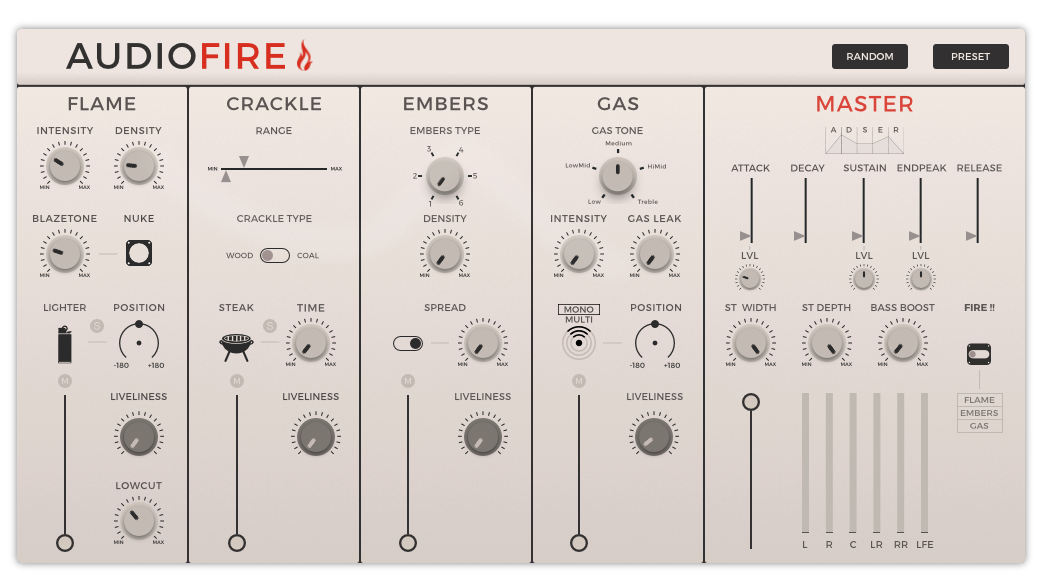
\includegraphics[scale=0.12]{AudioFire_screen.png}
	\caption{Audiofire: audio plug-in that recreates fire sound}
	\end{figure}
  \end{itemize}
\end{frame}

%-------------------------------------------------------
\subsection{Objective}
\begin{frame}{Introduction}{Objective}
%-------------------------------------------------------


  \begin{itemize}
          \item<1-> We are continuing the Audiogaming long project from 2015 (Emilie Abia, Lili Zheng, Quentin Biache)
\begin{block}{}
{\it Objective} : Synthesizing sounds from their spectrum with a $ FFT^{-1} $
	\begin{figure}
	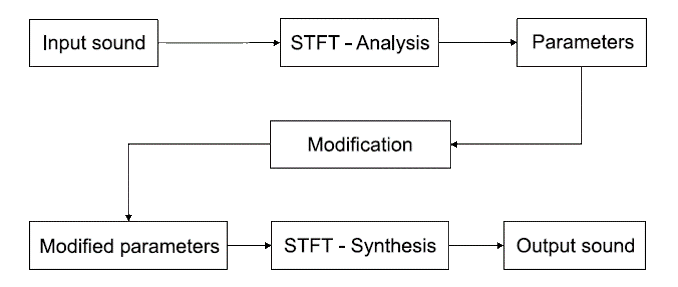
\includegraphics[scale=0.4]{Analysis_Synthesis.png}
	\caption{General approach for modifying a sound in the spectral domain}
	\end{figure}
\end{block}   
	\item<1-> We have to implement a new method of additive synthesis $\Rightarrow$ computationally very fast
  \end{itemize}
\end{frame}

%-------------------------------------------------------
\subsection{Context of the Project}
\begin{frame}{Introduction}{Context of the Project}
%-------------------------------------------------------

  \begin{itemize}
    \item<1-> 6 weeks only $\Rightarrow$ Focus on the synthesis method only.
   \begin{block}{}
	 Given codes in Python and Matlab from the 2015 project :
   \begin{itemize}
 	\item<1-> Python : Analysis estimator of sinus parameters and sinus generation with those parameters (only stationary)
 	\item<1-> Matlab : Some reasearch on the Non-stationary synthesis with the LUT of lobes
   \end{itemize}
   \end{block}   
	\item<1-> We made our own OOP codes in Python
	\item<1-> We have taken the analysis estimator code to test our final synthesis
  \end{itemize}
\end{frame}

%-------------------------------------------------------
\subsection{Work Environment and Project Management}
\begin{frame}{Introduction}{Work Environment}
%-------------------------------------------------------

\begin{figure}
	\centering
	
\includegraphics[scale=0.4]{all_softwares.png}
	\caption{ {\it PyCharm} as Python IDE , {\it Slack} to communicate,{\it GitHub} to stock the codes and have a versionning, {\it Freedcamp} to plan the project events }
\end{figure}
\end{frame}

\begin{frame}{Introduction}{Project Management : Gantt Chart}
%-------------------------------------------------------

\begin{figure}
	\centerline{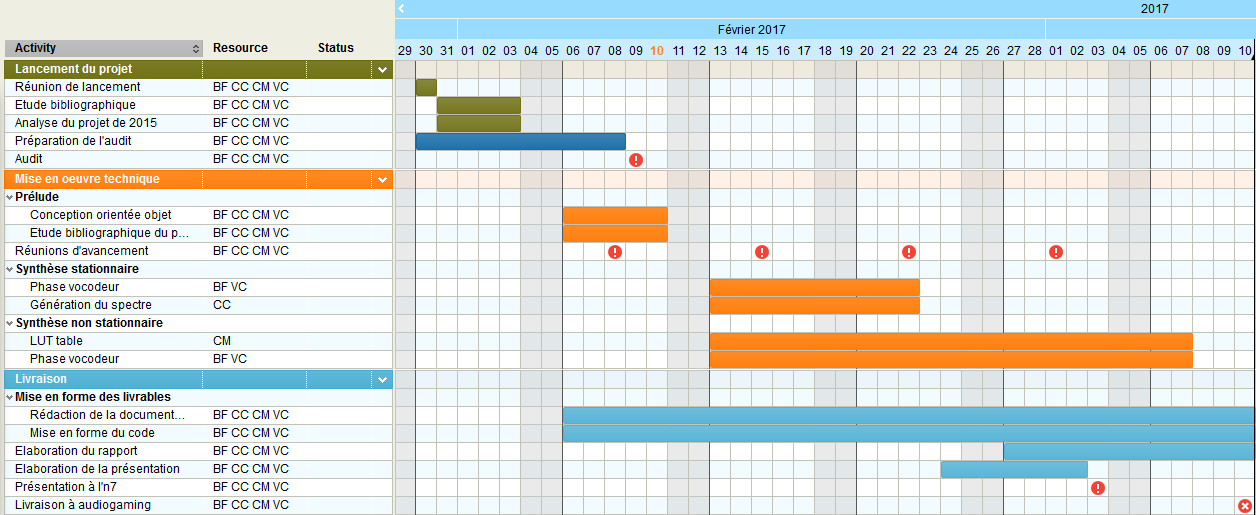
\includegraphics[scale=0.26]{Gantt.png}}
\end{figure}
\end{frame}

%-------------------------------------------------------
\section{Method Overview}
%-------------------------------------------------------
\subsection{Windowing}
\begin{frame}{Method Overview : Analysis}{Windowing}
%-------------------------------------------------------
\begin{figure}
	\centerline
	{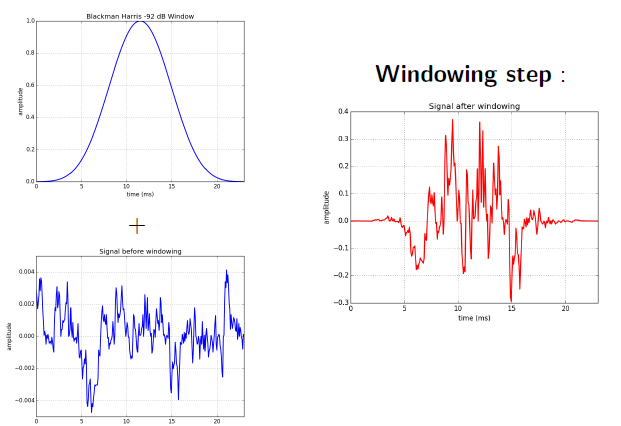
\includegraphics[scale=0.4]{slide1.png}}
	\caption{\it Windowing step}
\end{figure}
\end{frame}
%-------------------------------------------------------
\subsection{Peak Detection}
\begin{frame}{Method Overview : Analysis}{Peak Detection}
%-------------------------------------------------------
Peak detection and extraction of parameters by STPT (particular Short Time Fourier Transform):
\begin{figure}
	\centerline
	{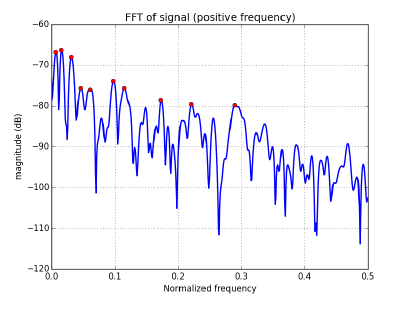
\includegraphics[scale=0.5]{slide2.png}}
	\caption{\it Peak detection}
\end{figure}
\end{frame}
%-------------------------------------------------------
\subsection{Result}
\begin{frame}{Method Overview : Synthesis}{Result}
%-------------------------------------------------------
Additive synthesis according to the parameters from the analysis:
\begin{figure}
	\centerline
	{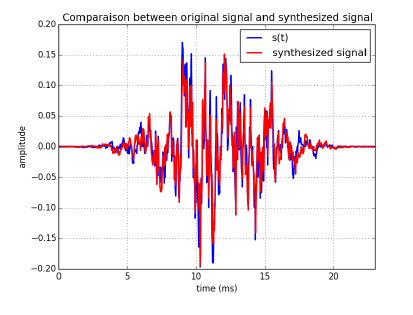
\includegraphics[scale=0.5]{synthesisstep.png}}
	\caption{\it Synthesized signal vs Original signal}
\end{figure}
\end{frame}
%-------------------------------------------------------
\section{The additive synthesis}
%-------------------------------------------------------
\subsection{General approach: The time domain}
\begin{frame}{The additive synthesis}{General approach: The time domain}
%-------------------------------------------------------
\begin{block}{}
The sound signal is represented as a sum of N sinusoids: \\
\centerline{
$ x(t) = \sum\limits_{n=1}^N a_{n} sin(2 \pi f_{n} t + \phi_{n})$}
\begin{itemize}
\item Very costly to implement
\item Impossible to compute in real-time
\end{itemize}
\end{block}
\begin{figure}
	\centerline
	{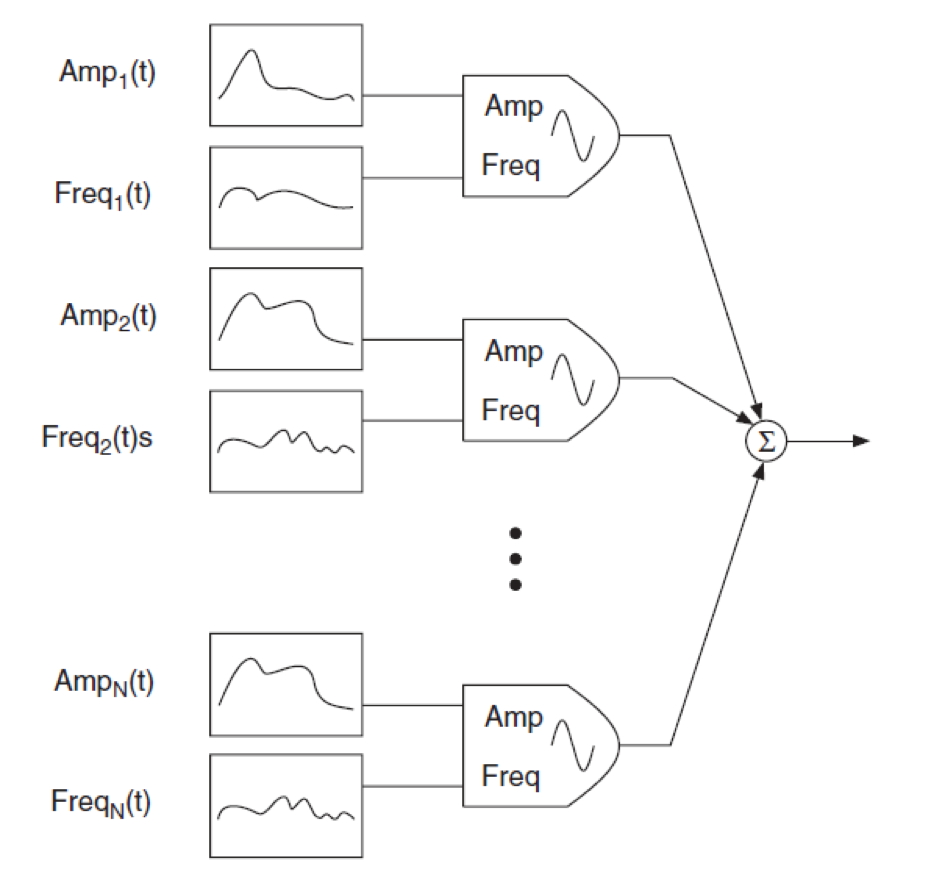
\includegraphics[scale=0.25]{additif.png}}
	\caption{\it The additive synthesis}
\end{figure}
\end{frame}

%-------------------------------------------------------
\subsection{General approach: The frequency domain}
\begin{frame}{The additive synthesis}{General approach: The frequency domain}
%-------------------------------------------------------
\begin{block}{}
We generate the sinusoids in frequency domain in order to reduce the computation time : \\

\begin{itemize}
\item Window the signal to maximize the energy in the main lobe
\item We only keep the main lobe for each sine (9 points)
\item We assume that the parameters (amplitude, frequency, phase) are already given by the analysis
\end{itemize}
\end{block}
\begin{figure}
	\centerline
	{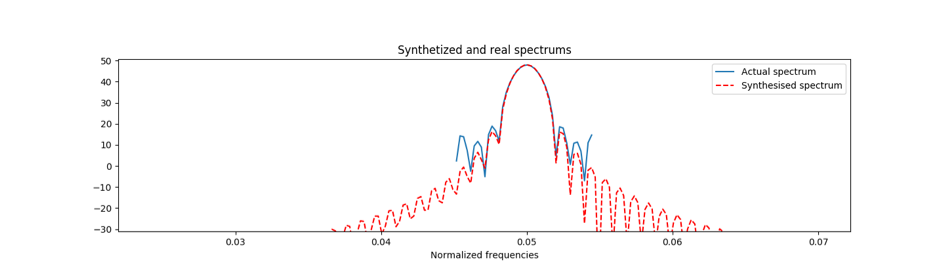
\includegraphics[scale=0.75]{lobe.png}}
	\caption{\it Windowed sine lobe}
\end{figure}
\end{frame}
%-------------------------------------------------------
\subsection{General approach: The frames}
\begin{frame}{The additive synthesis}{The frames}
%-------------------------------------------------------

The sound signal is  a frame-by-frame signal: \\

\begin{figure}

	{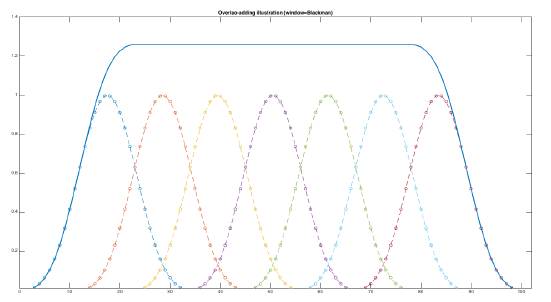
\includegraphics[scale=0.3]{overlap2.png}}
	\caption{\it Sum of small size Hanning windows}
\end{figure}
\begin{figure}
	{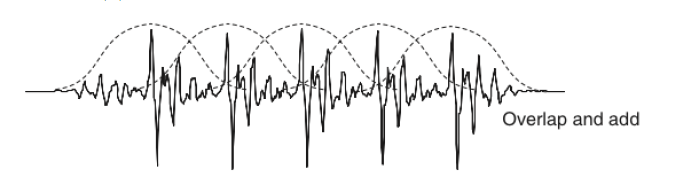
\includegraphics[scale=0.25]{overlap1.png}}
	\caption{\it Overlap and add}
\end{figure}
\end{frame}
%-------------------------------------------------------
\section{Stationary Signals}
%-------------------------------------------------------
\subsection{hjh}
\begin{frame}{Stationary Signals}{Source files}
%-------------------------------------------------------

\begin{block}{}

  \begin{itemize}
    \item {\tt }
    \item {\tt }
    \item {\tt }
    \item {\tt }
  \end{itemize}
\end{block}
\end{frame}

%-------------------------------------------------------
\subsection{}
\begin{frame}{}{}
%-------------------------------------------------------
  
  \begin{block}{n}
  \begin{itemize}    
    \item 
    \item 
  \end{itemize}
  \end{block}

  \begin{block}{}
  \begin{itemize}
     \item
     \item 
  \end{itemize}
  \end{block}
\end{frame}
     

%-------------------------------------------------------
\subsection{ }
\begin{frame}{}{ }
%-------------------------------------------------------

  
  \begin{itemize}
    \item 
    \item 
  \end{itemize}
 \end{frame}

%-------------------------------------------------------
\section{- }
\subsection{   -  }
\begin{frame}{- }{  -  }
%-------------------------------------------------------

  \begin{block}{ - }    
  \end{block}
  \begin{block}{-}
   \vspace{5pt} 
    \hspace{20pt}{-} 
    \begin{itemize}
    \item 
    \item
    \end{itemize}
  \end{block}

\end{frame}

%-------------------------------------------------------
\subsection{ }
\begin{frame}{ }{   }
%-------------------------------------------------------

\begin{block}{}
    \begin{itemize}
    \item 
    \item 
    \end{itemize} 
    
    \vspace{5pt} 
    

\end{block}
\end{frame}


{\1
\begin{frame}[plain,noframenumbering]
  \finalpage{Thank you!}
\end{frame}}

\end{document}